\documentclass[11pt]{article}

% ============================================================================
% DIMENSIONAL RIGIDITY: D = 3 FROM LINKING OF LOOPS, KEPLER STABILITY,
% AND MINIMAL DYADIC SYNCHRONIZATION
%
% Target: Discrete & Computational Geometry (primary)
% ============================================================================

\usepackage[utf8]{inputenc}
\usepackage[T1]{fontenc}
\usepackage{amsmath,amssymb,amsthm}
\usepackage{mathtools}
\usepackage{hyperref}
\usepackage{booktabs}
\usepackage{geometry}
\usepackage{tikz}
\usetikzlibrary{arrows.meta,positioning}
\geometry{margin=1in}

% Theorem environments
\newtheorem{theorem}{Theorem}[section]
\newtheorem{lemma}[theorem]{Lemma}
\newtheorem{proposition}[theorem]{Proposition}
\newtheorem{corollary}[theorem]{Corollary}
\newtheorem{definition}[theorem]{Definition}
\newtheorem{remark}[theorem]{Remark}
\newtheorem{example}[theorem]{Example}

% Notation
\newcommand{\Z}{\mathbb{Z}}
\newcommand{\R}{\mathbb{R}}
\newcommand{\N}{\mathbb{N}}
\newcommand{\Sph}{\mathbb{S}}
\newcommand{\lcmop}{\operatorname{lcm}}
\newcommand{\gcdop}{\gcd}
\newcommand{\lk}{\operatorname{lk}}
\newcommand{\Qcube}{Q_D}
\newcommand{\Gray}{\operatorname{Gray}}
\newcommand{\per}{\operatorname{per}}
\newcommand{\eps}{\varepsilon}

\title{Dimensional Rigidity: D=3 from Linking of Loops, Kepler Stability, and Minimal Dyadic Synchronization}

\author{%
Jonathan Washburn\thanks{Recognition Physics Institute, Austin, TX, USA. \texttt{jon@recognitionphysics.org}}
\and Milan Zlatanovi\'{c}\thanks{Faculty of Science and Mathematics, University of Ni\v{s}, Serbia. \texttt{zlatmilan@yahoo.com}}
\and Elshad Allahyarov\thanks{Case Western Reserve University, USA.}
}

\date{\today}

\begin{document}
\maketitle

\begin{abstract}
We give three mathematically precise constraints that each single out the spatial dimension $D=3$.
First, we show that an integer-valued linking invariant for disjoint oriented loops (embedded copies of $S^1$) exists only in $D=3$; this follows from Alexander duality, since for an embedded circle $K\subset \Sph^D$ the group $H_1(\Sph^D\setminus K)$ is isomorphic to $\Z$ if and only if $D=3$.
Second, for the $D$-dimensional Kepler potential determined by the Green's function of the Laplacian, $V_D(r)\propto -r^{2-D}$ (for $D\ge 3$), we derive the Binet equation and show that near-circular bound orbits are stable only for $D<4$, and are non-precessing (hence closed in the linearized regime) only for $D=3$.
Third, given a fixed odd ``gap'' period $45$, we show that the synchronization length $\lcmop(2^D,45)$ is minimized over $D\ge 3$ uniquely at $D=3$, where it equals $360$.
We also point to a Lean 4 formalization in the \texttt{IndisputableMonolith} library certifying the discrete (hypercube/Gray-cycle) and arithmetic (lcm) parts.
\end{abstract}

\noindent\textbf{Keywords:} dimension, linking number, Alexander duality, hypercube, Gray code, Kepler problem, apsidal precession

\noindent\textbf{MSC 2020:} 57K10, 55N40, 05C45, 70F05

% ============================================================================
\section{Introduction}
% ============================================================================

Why is physical space three-dimensional? There are many proposed answers (anthropic, dynamical, field-theoretic). In this note we record a compact rigidity phenomenon: several independent, cleanly stated mathematical requirements each force $D=3$.

To keep the argument modular, we isolate three constraints and note one optional sharp cross-check.
\begin{itemize}
  \item \textbf{(T) Topological loop-linking.} There should exist an integer-valued invariant measuring how two disjoint oriented loops link. We show this is possible only in $D=3$.
  \item \textbf{(K) Kepler stability from a point-source potential.} If one insists that the natural point-source potential in $\R^D$ (Green's function of the Laplacian) supports stable, non-precessing near-circular bound orbits, then $D=3$ is forced.
  \item \textbf{(S) Minimal dyadic synchronization with a fixed odd period.} If a system carries a dyadic cycle of length $2^D$ (e.g. a Gray-cycle on a $D$-cube) and an independent odd cycle of length $45$, then the synchronization length $\lcmop(2^D,45)$ grows exponentially in $D$. Among $D\ge 3$, its unique minimizer is $D=3$ (yielding $360$).
  \item \textbf{(C) Spinor/gauge structure (optional cross-check).} Requiring 2-component complex spinors together with a non-abelian simple rotation cover $\mathrm{Spin}(D)$ also singles out $D=3$ (since $\mathrm{Cl}_3\cong M_2(\mathbb{C})$ and $\mathrm{Spin}(3)\cong \mathrm{SU}(2)$). We do not develop this here.
\end{itemize}

The constraints above are intentionally sharp: each one already characterizes $D=3$. We use ``independent'' in the sense of originating from distinct mathematical/physical sectors, not as a set-theoretic independence claim. (If one prefers a nontrivial intersection-of-allowed-sets formulation, each condition can be weakened to allow multiple dimensions before intersecting; we do not pursue that variant here.)

The proofs use standard tools (Alexander duality; Binet equation and linearization; elementary number theory), and we include a diagram of a canonical Gray $8$-cycle on the cube.

\smallskip
\noindent\textbf{Motivating context.} In the broader Recognition Science program, the dyadic period $2^D$ arises from a ledger traversal on a $D$-dimensional binary register, while the odd period $45$ appears as a ``gap'' index; the accepted Recognition Geometry paper provides a measurement-first axiomatic setting for this viewpoint (see~\cite{RG2026}). Nothing in the proofs below depends on that framework.

% ============================================================================
\section{Preliminaries: the hypercube and Gray cycles}
% ============================================================================

\begin{definition}[Hypercube graph]
For $D\in\N$, the $D$-dimensional hypercube graph $Q_D$ has vertex set $\{0,1\}^D$ with an edge between two vertices iff they differ in exactly one coordinate.
\end{definition}

\begin{definition}[Gray cycle]
A \emph{Gray cycle} on $Q_D$ is a Hamiltonian cycle on $Q_D$, equivalently a cyclic ordering of the $2^D$ binary strings where consecutive strings differ in one bit.
\end{definition}

\begin{proposition}[Existence of Gray cycles]
For every $D\ge 1$, $Q_D$ admits a Gray cycle.
\end{proposition}

\begin{proof}[Construction sketch]
Let $\Gray_1 = (0,1)$. Given a Gray cycle $\Gray_D$ on $\{0,1\}^D$, form a Gray cycle on $\{0,1\}^{D+1}$ by
\[
\Gray_{D+1} := (0\Gray_D,\; 1\overline{\Gray_D}),
\]
where $0\Gray_D$ means prepend a $0$ to each word in $\Gray_D$, and $\overline{\Gray_D}$ denotes the reverse traversal. This yields a Hamiltonian cycle on $Q_{D+1}$ with one-bit steps.
\end{proof}

\begin{remark}
The existence of Gray codes is classical (see~\cite{Gray1953,Savage1997}). We only need that the natural dyadic period associated to a full traversal is $2^D$.
\end{remark}

\begin{definition}[Dyadic period]
We define the dyadic period of dimension $D$ as $\per(D):=2^D$.
\end{definition}

\begin{figure}[t]
\centering
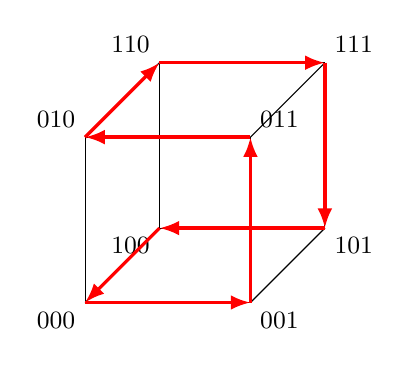
\begin{tikzpicture}[scale=1.05, every node/.style={font=\small}]
  % Cube projection
  \coordinate (A)  at (0,0);
  \coordinate (B)  at (2,0);
  \coordinate (C)  at (2,2);
  \coordinate (D)  at (0,2);
  \coordinate (Ap) at (0.9,0.9);
  \coordinate (Bp) at (2.9,0.9);
  \coordinate (Cp) at (2.9,2.9);
  \coordinate (Dp) at (0.9,2.9);

  \draw (A)--(B)--(C)--(D)--cycle;
  \draw (Ap)--(Bp)--(Cp)--(Dp)--cycle;
  \draw (A)--(Ap) (B)--(Bp) (C)--(Cp) (D)--(Dp);

  % Labels: bottom square (z=0)
  \node[below left] at (A) {$000$};
  \node[below right] at (B) {$001$};
  \node[above right] at (C) {$011$};
  \node[above left] at (D) {$010$};
  % Labels: top square (z=1)
  \node[below left] at (Ap) {$100$};
  \node[below right] at (Bp) {$101$};
  \node[above right] at (Cp) {$111$};
  \node[above left] at (Dp) {$110$};

  % Highlight the canonical Gray 8-cycle
  \draw[very thick, red, -{Latex[length=2.5mm]}] (A) -- (B);
  \draw[very thick, red, -{Latex[length=2.5mm]}] (B) -- (C);
  \draw[very thick, red, -{Latex[length=2.5mm]}] (C) -- (D);
  \draw[very thick, red, -{Latex[length=2.5mm]}] (D) -- (Dp);
  \draw[very thick, red, -{Latex[length=2.5mm]}] (Dp) -- (Cp);
  \draw[very thick, red, -{Latex[length=2.5mm]}] (Cp) -- (Bp);
  \draw[very thick, red, -{Latex[length=2.5mm]}] (Bp) -- (Ap);
  \draw[very thick, red, -{Latex[length=2.5mm]}] (Ap) -- (A);
\end{tikzpicture}
\caption{A standard Gray $8$-cycle on $Q_3$: $000\to001\to011\to010\to110\to111\to101\to100\to000$.}
\label{fig:gray8}
\end{figure}

% ============================================================================
\section{Constraint (T): an integer linking invariant for loops forces \texorpdfstring{$D=3$}{D=3}}
% ============================================================================

We record the clean algebraic-topological fact behind ``linking of loops is special to three dimensions.''

\begin{definition}[Linking number via homology]
Let $K\subset \Sph^3$ be an oriented embedded circle, and let $L\subset \Sph^3\setminus K$ be another oriented embedded circle disjoint from $K$.
By Alexander duality, $H_1(\Sph^3\setminus K)\cong \Z$. The \emph{linking number} $\lk(L,K)\in\Z$ is the image of $[L]\in H_1(\Sph^3\setminus K)$ under this identification.
\end{definition}

\begin{theorem}[Alexander duality computation]\label{thm:alex-dual}
Let $D\ge 2$ and let $K\subset \Sph^D$ be an embedded circle. Then
\[
H_1(\Sph^D\setminus K) \cong \widetilde H^{D-2}(S^1).
\]
In particular,
\[
H_1(\Sph^D\setminus K)\cong\begin{cases}
\Z & D=3,\\
0 & D\ne 3.
\end{cases}
\]
\end{theorem}

\begin{proof}
Alexander duality gives $\widetilde H_i(\Sph^D\setminus K)\cong \widetilde H^{D-i-1}(K)$ for compact, locally contractible $K\subset \Sph^D$ (see~\cite[Ch.~3]{Hatcher}). Taking $i=1$ and $K\simeq S^1$, we obtain $\widetilde H_1(\Sph^D\setminus K)\cong \widetilde H^{D-2}(S^1)$.
Since $\widetilde H^{j}(S^1)$ is $\Z$ only for $j=1$ and is $0$ otherwise, the claim follows.
\end{proof}

\begin{corollary}[Topological rigidity for loop-linking]\label{cor:linking-only-3}
An integer-valued linking number for disjoint oriented loops, defined via $H_1(\Sph^D\setminus K)$, can exist only when $D=3$.
\end{corollary}

\begin{remark}[General intersection dimension]
From the perspective of geometric topology, linking numbers arise as intersection numbers of a bounding chain. If $M^p$ and $N^q$ are disjoint closed oriented submanifolds in $\R^D$, a generic chain $C^{p+1}$ with $\partial C = M$ will intersect $N^q$ stably at isolated points if and only if:
\[
(p+1) + q = D \implies p+q+1 = D.
\]
For 1D observables (worldlines or loops), we have $p=q=1$, which forces $1+1+1=D$, uniquely selecting $D=3$. This places the result in the standard hierarchy of intersection invariants (e.g., points link loops in $D=2$, surfaces link surfaces in $D=5$).
\end{remark}

\begin{example}[Hopf link]
In $\Sph^3$ there exist disjoint loops with $\lk=1$, e.g. the Hopf link. This shows the invariant is nontrivial in $D=3$ (see~\cite{Rolfsen}).
\end{example}

% ============================================================================
\section{Constraint (K): Kepler stability from a point-source potential}
% ============================================================================

We next record a dimension-sensitive computation showing that $D=3$ is singled out by stability and non-precession for the Kepler problem induced by the Laplacian Green's function.

\subsection{The \texorpdfstring{$D$}{D}-dimensional Kepler potential}
For $D\ge 3$, the fundamental solution of the Laplacian implies a point-source potential of the form
\begin{equation}\label{eq:kepler-potential}
V_D(r) = -\mu\, r^{2-D},\qquad r>0,
\end{equation}
for a constant $\mu>0$ (we only use the power $2-D$).

\subsection{Binet equation and linearization}
Motion in a central potential is confined to a plane, so we may use polar coordinates $(r,\theta)$ and set $u(\theta)=1/r(\theta)$.
For a radial force $F(r)=-V_D'(r)$, the Binet equation reads
\begin{equation}\label{eq:binet}
u''(\theta)+u(\theta) = -\frac{m}{\ell^2 u(\theta)^2}\,F\bigl(1/u(\theta)\bigr),
\end{equation}
where $m$ is the mass and $\ell$ is the (scalar) angular momentum.

\begin{lemma}[Binet form for $V_D$]\label{lem:binet-kepler}
For the potential~\eqref{eq:kepler-potential} with $D\ge 3$, the Binet equation becomes
\begin{equation}\label{eq:binet-kepler}
u'' + u = \beta\, u^{D-3},
\end{equation}
for some constant $\beta>0$.
\end{lemma}

\begin{proof}
Compute $V_D'(r) = -\mu(2-D) r^{1-D} = \mu(D-2) r^{1-D}$, so the attractive radial force is
$F(r)=-V_D'(r) = -\mu(D-2) r^{1-D}$.
Substituting $r=1/u$ gives $F(1/u)=-\mu(D-2)u^{D-1}$. Plugging into~\eqref{eq:binet} yields
$u''+u = \frac{m\mu(D-2)}{\ell^2}\,u^{D-3}$.
Set $\beta = \frac{m\mu(D-2)}{\ell^2}>0$.
\end{proof}

\begin{proposition}[Stability and apsidal angle]\label{prop:apsidal}
Assume $D\ge 3$ and consider a circular orbit solution $u\equiv u_0>0$ of~\eqref{eq:binet-kepler}. Linearizing $u=u_0+\eps$ around $u_0$ yields
\[
\eps'' + (4-D)\,\eps = 0.
\]
Consequently:
\begin{enumerate}
  \item For $D\ge 5$, circular orbits are linearly unstable.
  \item For $D=4$, circular orbits are marginal ($\eps''=0$).
  \item For $D=3$, circular orbits are stable with angular frequency $1$ in the $\theta$ variable; the apsidal angle is exactly $\pi$, so near-circular bound orbits are non-precessing.
\end{enumerate}
\end{proposition}

\begin{proof}
A circular orbit $u\equiv u_0$ satisfies $u_0=\beta u_0^{D-3}$, hence $\beta=u_0^{4-D}$.
Write $u=u_0+\eps$ with $|\eps|\ll 1$ and expand:
\[
\beta(u_0+\eps)^{D-3} = \beta u_0^{D-3} + \beta(D-3)u_0^{D-4}\eps + O(\eps^2).
\]
Using $\beta u_0^{D-3}=u_0$ and $\beta u_0^{D-4}=1$, the linearized equation becomes
$\eps''+\eps=(D-3)\eps$, i.e. $\eps''+(4-D)\eps=0$.
The conclusions follow by inspecting the sign of $4-D$. For $D=3$, solutions are periodic with frequency $1$, so the radial oscillation period equals $2\pi$ in $\theta$, giving apsidal angle $\pi$ (no precession in the linear regime).
\end{proof}

\begin{remark}
In $D=3$ the Kepler problem is exactly integrable and yields closed conics; Bertrand's theorem characterizes the Kepler and harmonic oscillator potentials as the only central potentials for which all bounded orbits are closed~\cite{Bertrand1873}.
\end{remark}

\begin{remark}[The case $D=2$]
In $D=2$ the Laplacian Green's function yields a logarithmic potential $V_2(r)\propto \log r$ rather than a power law. The Binet analysis above is stated for $D\ge 3$; in particular, the no-precession phenomenon recovered in Proposition~\ref{prop:apsidal} is specific to $D=3$ within the Laplacian point-source family.
\end{remark}

% ============================================================================
\section{Constraint (S): minimal synchronization with an odd period}
% ============================================================================

Fix an odd integer $N$ (in the RS-motivated application, $N=45$). Define the synchronization length
\[
S(D):=\lcmop(2^D, N).
\]
When $N$ is odd, $\gcdop(2^D,N)=1$, so $S(D)=N\cdot 2^D$.

\begin{lemma}\label{lem:lcm}
For every $D\ge 0$, $\gcdop(2^D,45)=1$ and hence
\[
\lcmop(2^D,45)=45\cdot 2^D.
\]
\end{lemma}

\begin{proof}
Since $45$ is odd, it shares no prime factor with $2^D$. Thus $\gcdop(2^D,45)=1$ and $\lcmop(2^D,45)=2^D\cdot 45$.
\end{proof}

\begin{proposition}[Unique minimizer over $D\ge 3$]\label{prop:min}
Let $S(D):=\lcmop(2^D,45)$. Then $S(D)$ is strictly increasing in $D$ and, among integers $D\ge 3$, the unique minimizer is $D=3$ with $S(3)=360$.
\end{proposition}

\begin{proof}
By Lemma~\ref{lem:lcm}, $S(D)=45\cdot 2^D$. Hence $S(D+1)=2S(D)$, so $S$ is strictly increasing.
In particular, for $D\ge 3$ we have $S(D)\ge S(3)=45\cdot 8=360$, with equality iff $D=3$.
\end{proof}

\begin{remark}
This ``minimal synchronization'' constraint is only meaningful when paired with an independent lower bound $D\ge 3$ (e.g. from Constraint~(T) or (K)).\linebreak
In the RS documents, $45$ is additionally motivated as the triangular number $T_9=1+\cdots+9$; the Lean module
\texttt{IndisputableMonolith.Gap45.}\allowbreak\texttt{PhysicalMotivation} records that viewpoint.
\end{remark}

% ============================================================================
\section{Combined rigidity theorem}
% ============================================================================

\begin{theorem}[Dimensional rigidity at $D=3$]\label{thm:combined}
Each of the constraints (T), (K), and (S) forces $D=3$. In particular, if any two of these conditions are required simultaneously, they are compatible only in dimension three.
\end{theorem}

\begin{proof}
Constraint~(T) gives $D=3$ by Corollary~\ref{cor:linking-only-3}. Constraint~(K) gives $D=3$ by Proposition~\ref{prop:apsidal}. Constraint~(S) gives that among $D\ge 3$ the unique minimizer is $D=3$ by Proposition~\ref{prop:min}.
\end{proof}

% ============================================================================
\section{Lean 4 formalization (discrete and arithmetic components)}
% ============================================================================

Parts of the discrete and arithmetic content of this note are mechanized in Lean 4. The code lives in the \texttt{IndisputableMonolith} library.

\subsection*{Verified items}
\begin{itemize}
  \item \textbf{Gray 8-cycle on $Q_3$.} In \texttt{IndisputableMonolith/Patterns/}\texttt{GrayCycle.lean}:
  \begin{verbatim}
def grayCycle3Path : Fin 8 -> Pattern 3 := ...
theorem grayCycle3_bijective : Function.Bijective grayCycle3Path := by ...
theorem grayCycle3_oneBit_step : forall i : Fin 8, OneBitDiff ... := by ...
  \end{verbatim}
  \item \textbf{Synchronization identity and lcm forcing.}\linebreak
  In \texttt{IndisputableMonolith/RecogSpec/}\texttt{Bands.lean}:
  \begin{verbatim}
theorem lcm_pow2_45_eq_iff (D : Nat) :
  Nat.lcm (2^D) 45 = 360 <-> D = 3 := by ...
  \end{verbatim}
  \item \textbf{Dimension forced from ``cover + sync'' predicate.}\linebreak
  In \texttt{IndisputableMonolith/Verification/}\texttt{Dimension.lean}:
  \begin{verbatim}
theorem rs_counting_gap45_absolute_iff_dim3 :
  RSCounting_Gap45_Absolute D <-> D = 3 := by ...
  \end{verbatim}
\end{itemize}

\begin{remark}
The topological and dynamical constraints (Alexander duality; Kepler stability) are standard mathematics and are presented here as conventional proofs; they are not currently the focus of the Lean mechanization.
\end{remark}

% ============================================================================
\section{Scope and limitations}

\begin{itemize}
  \item \textbf{Topology.} Constraint~(T) is about \emph{loop-loop} integer linking; other dimensions support other linking phenomena (e.g. $S^2$--$S^2$ linking in $D=5$). The claim here is that loops enjoy an integer linking invariant only in $D=3$.
  \item \textbf{Dynamics.} Constraint~(K) assumes the point-source potential is the Laplacian Green's function. Other potentials may behave differently; the point is that the most canonical ``no free scale'' potential family is dimension-sensitive, and the Kepler/non-precession behavior is uniquely $D=3$.
  \item \textbf{Arithmetic.} Constraint~(S) treats the odd period $45$ as an external input. The rigorous statement is a minimality fact: among $D\ge 3$, synchronization overhead grows like $2^D$, and the unique minimizer is $D=3$.
\end{itemize}

\section{Conclusion}
% ============================================================================

We highlighted three independent mechanisms that single out $D=3$: loop-linking via $H_1$ of the complement, stability and non-precession for the Laplacian point-source Kepler potential, and minimal dyadic synchronization with an odd period.

\section*{Acknowledgments}
We thank the Mathlib community for the Lean 4 ecosystem.

% ============================================================================
% REFERENCES
% ============================================================================

\begin{thebibliography}{99}

\bibitem{RG2026}
J.~Washburn, M.~Zlatanovi\'{c}, and E.~Allahyarov,
\emph{Recognition Geometry},
Axioms (2026).
DOI: \href{https://doi.org/10.3390/1010000}{10.3390/1010000}.

\bibitem{Hatcher}
A.~Hatcher,
\emph{Algebraic Topology},
Cambridge University Press, 2002.

\bibitem{Rolfsen}
D.~Rolfsen,
\emph{Knots and Links},
Publish or Perish, 1976.

\bibitem{Gray1953}
F.~Gray,
\emph{Pulse Code Communication},
U.S.\ Patent 2,632,058 (1953).

\bibitem{Savage1997}
C.~Savage,
\emph{A Survey of Combinatorial Gray Codes},
SIAM Review \textbf{39} (1997), 605--629.

\bibitem{Bertrand1873}
J.~Bertrand,
\emph{Th\'{e}or\`{e}me relatif au mouvement d'un point attir\'{e} vers un centre fixe},
Comptes Rendus Acad. Sci. Paris (1873).

\end{thebibliography}

\end{document}

